 % !TeX spellcheck = en_US
That cells communicate with one another is an obvious necessity for multicellular organisms to exists, but it is also a well established fact for microbes. Cell types within an animal have to grow following a carefully defined choreography or risk spiraling into chaos. Every cell in our body  subordinates its cell cycle and most of its biochemical  processes to the dictates of messenger signals such as hormones. Only thus, can every cell type position itself where it is needed and perform its functions. One cell acting out of sync, can lead to fatal consequences such as tumors and eventually kill the organism. Such precise synchronization between components is not easy to achieve, as we have learned after more than a century of developing complex machines. Just as micro-electronics has developed a wide variety of integrated circuits, sensors and component in general, cells must have equally sophisticated circuits that process complex signals. If electronic circuits must include switches, timers, motion detectors and relays, biological circuits must be able to switch genes on and off, detect infection, respond to the proximity of other cells and carry a signal from one point of the body to another. In both cases, electronics and cell biology, these elements must be re-usable. Electronic components are mass produced and then combined in different forms to produce machines. Biological components, are also re-used by evolution and we find the same combination of genes or proteins performing different functions within the same cell or in different ones. Once a group of proteins proves to be able to fulfill a function, it is often duplicated and co-opted to play a different role. Such is the case of two component systems, with a sensor kinase that detects a stimulus and a response protein that transmit the signal. A single bacteria can have more that a dozen variants of this system to detect and respond to different stimuli.

Many critical functions within a cell depend on such circuits and many diseases are the result of failures in their functioning so any attempt at building synthetic biological components or healing these diseases are conditioned by our ability to understand the dynamics of their associated components.

\section{Biological circuits}

With biological circuit, we mean a group of biological components (proteins, DNA, RNA, \dots ) that work together to perform a function. To define its behavior, we can say that our circuit is a system that, when confronted with a certain input, will produce a certain output. In biology we often replace the concepts input and output with \textbf{stimulus} and \textbf{response}, respectively.

We are used to talk about electronic circuits by describing their input output response. A doorbell, for instance, is a button that makes a sound when it is pressed and stops making any sound whenever it is released.  A switch is also a button, but once we press it, it changes to a new state and stays in it. For instance, when we enter a room and press the light switch, the light goes on. After releasing the switch, the light stays on and will only turn off if we press the switch again. From these simple examples we can move on to more complex circuits. A  timer is a circuit that sends a signal after a certain amount of time has passed, a relay is like a switch but it reacts to an electric current instead of physical pressure. We can use relays to open a garage door remotely. We can even combine several simple elements in a single machine. We can use an infra-red sensor to detect the garage remote, the sensor can then send a signal to a relay that opens the garage door and forwards the signal to a timer that after ninety seconds, sends a signal back to the relay to shut the door. Can we imagine the biological counterparts to these components?

\paragraph{Sensors} Cells have many different sensors and some cell types within a body are sensors themselves. We have already mentioned two-component systems in bacteria, which contain sensors able to detect signals out of the cell -- e.g. hormones, food, poisons, \dots -- or in the cell -- levels of acetyl-CoA, osmotic pressure in the membrane, \dots. But there are many more molecules within a cell that can detect signals. Practically every variable that is relevant to cell biology is tracked by one sensor or another: alternative carbon sources can be detected by repressors or activators of the relevant operon, neurotransmitters are detected or imported into post-synaptic neurons  and converted in action potentials, peptidic hormons like insulin are detected by receptors in the surface of the cell while many steroid hormones are imported in the cell where they attach to some protein that binds to DNA \dots 

\paragraph{Signal transduction} The many different signals perceived by the sensors has to be translated to some standard signal. Unlike electronic components, which convert everything to electricity, cellular signals have a wider diversity. A typical mean to transmit signals within the cell is the phosphorylation state of a protein, but other alternatives exist such as methylation states, ion concentrations -- e.g. $K^+$, $Ca^{2+}$, \dots -- or second messengers such as cyclic AMP.
\paragraph{Signal processing} The same signal can trigger different responses in different organisms or even in different cells within the same organism. Liver cells, for instance, respond to insulin by releasing glucose into the bloodstream, while most other cells respond by increasing their glucose uptake. One way of achieving this, is having different components able to respond to a certain signal. Some circuits may show a proportional response to a certain stimulus, others may have an all or nothing response -- e.g. triggering fever when inflammation indicators exceed a certain threshold -- and some systems may behave as a switch, changing their state when a signal is received and staying in this new state. An example of the latter would be cell differentiation, when a signal during embryonic development permanently changes the type of a cell and the genes it expresses.

\paragraph{Other behaviors} The wide diversity of cell behaviors found in nature is proof of the unlimited creativity with which natural selection has been able tweak biological circuits. Molecular clocks keep track of time within the cells and periodic systems, such as those underlying circadian rythms synchronize practically every aspect of our metabolism to the dictates of the  external clock that is sunlight. Some circuits can modify the behavior of sensors. Temperature sensors in the skin of mammals, for instance, do not respond to temperature itself, but rather to changes in it. In other words, the intensity of the signal of a temperature receptor is proportional to the derivative of temperature with respect to time and the same behavior is observed by food receptors governing chemotaxis in bacteria. This type of behavior is called adaptation. 


In this chapter we will see and study several examples of how to build different types of circuits with just a few components. we will build linear transducers, interrupters, switches, oscillators -- clocks-- and circuits able to show adaptation.

\subsection{Linear response}

\begin{figure}
	\begin{center}
		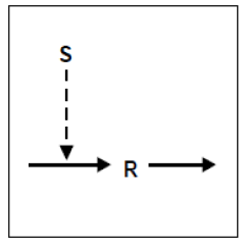
\includegraphics[width=0.3\textwidth]{BiocircLinear}
	\end{center}
	\caption{ ... }
	\label{fig:bclin}
\end{figure}
\subsection{Saturated response}
\begin{figure}
	\begin{center}
		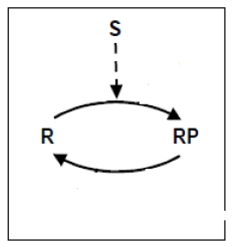
\includegraphics[width=0.3\textwidth]{BiocircMM}
	\end{center}
	\caption{ ... }
	\label{fig:bcsat}
\end{figure}
\subsection{Buzzer (interrupter)}
\begin{figure}
	\begin{center}
		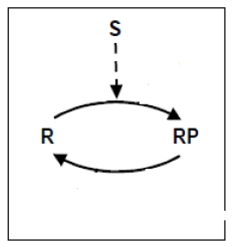
\includegraphics[width=0.3\textwidth]{BiocircMM}
	\end{center}
	\caption{ ... }
	\label{fig:bcsigmoid}
\end{figure}
\subsection{Switch}
\subsection{Oscillators (clocks)}
\subsection{Adaptation}

\begin{figure}
	\begin{center}
		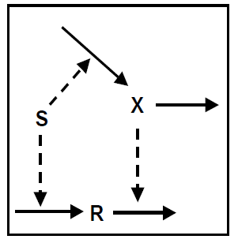
\includegraphics[width=0.3\textwidth]{BiocircAdapt}
	\end{center}
	\caption{ ... }
	\label{fig:bcadapt}
\end{figure}

\subsection{Quorum sensing}